\documentclass[12pt, a4paper, oneside]{article}
\usepackage{amsmath, amsthm, subcaption, float,amssymb, bm, graphicx, hyperref, mathrsfs, geometry, listings, xcolor}

\title{\large\textbf{STA2002 - Homework 5}}
\author{Xue Zhongkai 122090636}
\date{}
\linespread{1.5}
\geometry{a4paper, scale=0.9}
\newcounter{problemname}
\newenvironment{problem}{\stepcounter{problemname}\par\noindent\textsc{Problem \arabic{problemname}. }}{\\\par}

\begin{document}
\maketitle

% Problem 1
\begin{problem}
    \\
    (a) With relative formulas, the ANOVA table is as follows:  
    \begin{table}[H]
        \centering
        \begin{tabular}{|l|c|c|c|c|}
        \hline
        \textbf{Source} & SS        & df  & MS         & F        \\ \hline
        Brand (A)       & 1387.50   & 3   & 462.50     & 0.676    \\ \hline
        Surface (B)     & 2888.08   & 2   & 1444.04    & 2.109    \\ \hline
        Interaction     & 8100.25   & 6   & 1350.04    & 1.972    \\ \hline
        Error           & 8216.00   & 12  & 684.67     &  ---     \\ \hline
        \textbf{Total}  & 20591.83  & 23  &  ---       &  ---     \\ \hline
        \end{tabular}
    \end{table}
    \noindent (b)(c)(d) And here are the tests:
    \begin{table}[H]
        \centering
        \begin{tabular}{|c|l|c|}
        \hline
        \textbf{Hypotheses}    & \qquad Contents       & Thresholds                    \\ \hline
        $H_A$                  & No row effect.        & $F_{0.05}(3, 12) = 3.490 $    \\ \hline
        $H_B$                  & No column effect.     & $F_{0.05}(2, 12) = 3.885 $    \\ \hline
        $H_{AB}$               & No interaction.       & $F_{0.05}(6, 12) = 2.996 $    \\ \hline
        \end{tabular}
    \end{table}
    \noindent From above, we fail to reject $H_A$, $H_B$ and $H_{AB}$.\\
    That is, it is reasonable to believe there is \textbf{NO row effect}, \textbf{NO column effect} and \textbf{NO interaction}.
\end{problem}

% Problem 2
\begin{problem}
    \\
    (a) By LSE, we first figure out
    $$ S_{xy} = \sum y_i x_i - \frac{\sum{y_i} \sum{x_i}}{n} = 1083.67 - \frac{12.75 \times 1478}{20} = 141.445$$
    $$ S_{xx} = \sum{x_i^2}-\frac{(\sum x_i)^2}{n} = 143215.8-\frac{(1478)^2}{20} = 33,991.6$$
    Further the intercept and slope in the simple linear regression model are 
    $$ \hat{\beta_1} = \frac{S_{xy}}{S_{xx}} 
                     = \frac{141.445}{33,991.6}
                     = 4.161 \times 10^{-3}
    $$
        Since $\overline{y} = \frac{\sum y_i}{n} = \frac{12.75}{20}=0.6375$, $\overline{x} = \frac{\sum x_i}{n} = \frac{1478}{20}=73.9$,
    $$ \hat{\beta_0} = \overline{y} - \hat{\beta_1} \overline{x} = 0.6375 - 4.161 \times 10^{-3} \cdot 73.9 = 0.3300$$
    \textbf{That is, the regression line is} $$ \hat{y} = 4.161 \times 10^{-3} \cdot x + 0.3300 $$
    \textbf{The graph is as follows: }
    \begin{figure}[H]
        \centering
        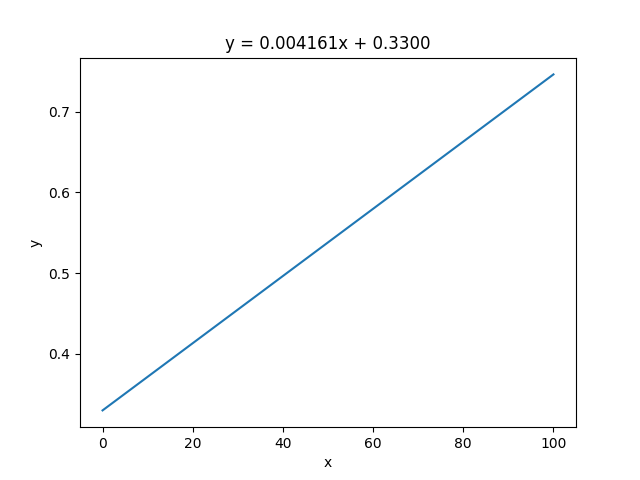
\includegraphics[width=0.5\textwidth]{fig_1.png}
    \end{figure}
    \noindent To estimate the $\sigma^2$,
    $$ SS_T = \sum y_i^2 - n \bar{y}^2 = 8.86 - 20 \times 0.6375^2 = 0.7319$$
    $$ SS_E = SS_T - \hat{\beta_1} S_{xy} = 0.1433$$
    \textbf{We have estimated variance to be }
    $$ \hat{\sigma^2} = \frac{SS_E}{n-2} = \frac{0.1433}{20-2} = 7.9611 \times 10^{-3}$$
    \\
    (b) For the surface temperature as 85F, 
    $$ \hat{y} = 4.161 \times 10^{-3} \cdot 85 + 0.3300 \approx 0.6837$$
    \textbf{The pavement deflection would be 0.6837 at the given temperature.}
    \\
    (c) For the temperature as 90F, we have the mean pavement deflection
    $$ \mu_{Y|x_0} = \beta_0 + \beta_1 x_0 = 4.161 \times 10^{-3} \cdot 90 + 0.3300 \approx 0.7045$$
    \textbf{The mean of the pavement deflection would be 0.7045 at the given temperature.}
    \\
    (d) For the regression line $ \hat{y} = 4.161 \times 10^{-3} \cdot x + 0.3300$, \\
    1F change in surface temperature will result in \textbf{a change of $4.161 \times 10^{-3}$ in mean pavement deflection}.
\end{problem}

% Problem 3
\begin{problem}
    \\
    (a) We use python codes to figure out means and variances. \\
    With codes below:
    \begin{figure}[H]
        \centering
        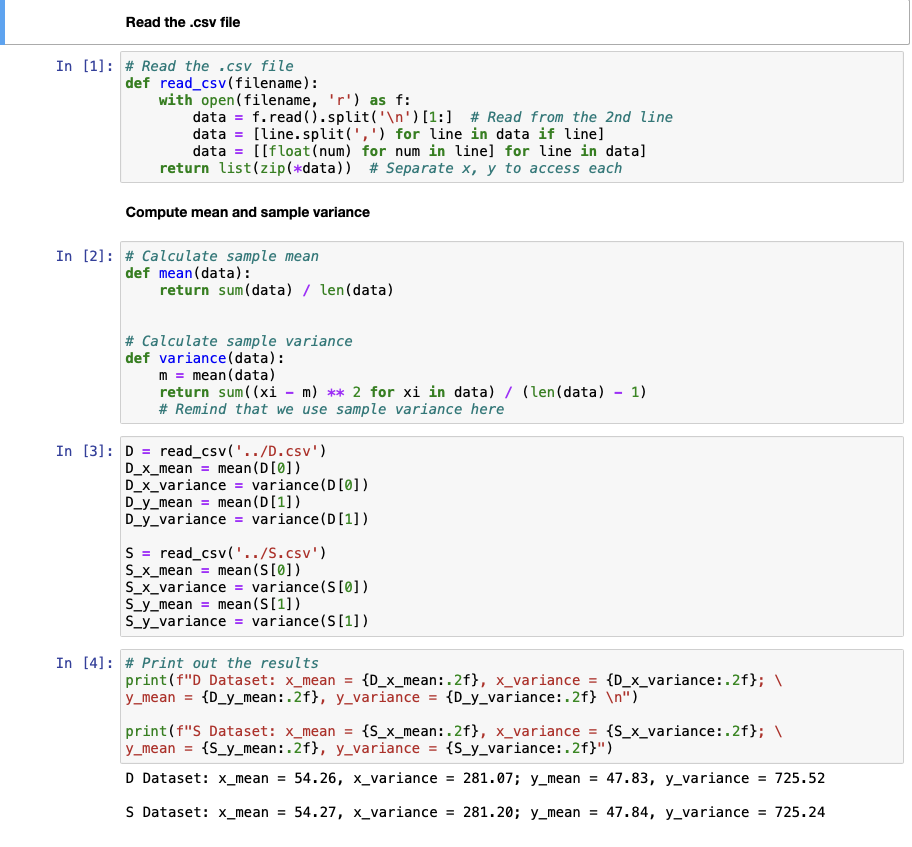
\includegraphics[width=0.8\textwidth]{MnV_code.png}
    \end{figure}    
    \noindent \textbf{We figure out the results:}
    \begin{table}[H]
        \centering
        \begin{tabular}{|l|c|c|c|c|}
        \hline
                        & $x^D$    & $x^S$     & $y^D$     & $y^S$       \\ \hline
        Sample mean     & 54.26    & 54.27     & 47.83     & 47.84       \\ \hline
        Sample variance & 281.07   & 281.20    & 725.52    & 725.24      \\ \hline
    \end{tabular}
    \end{table}
    \noindent (b) Given the linear regression model $y = \beta(x-\bar{x}) + \alpha $, \\
    \begin{figure}[H]
        \centering
        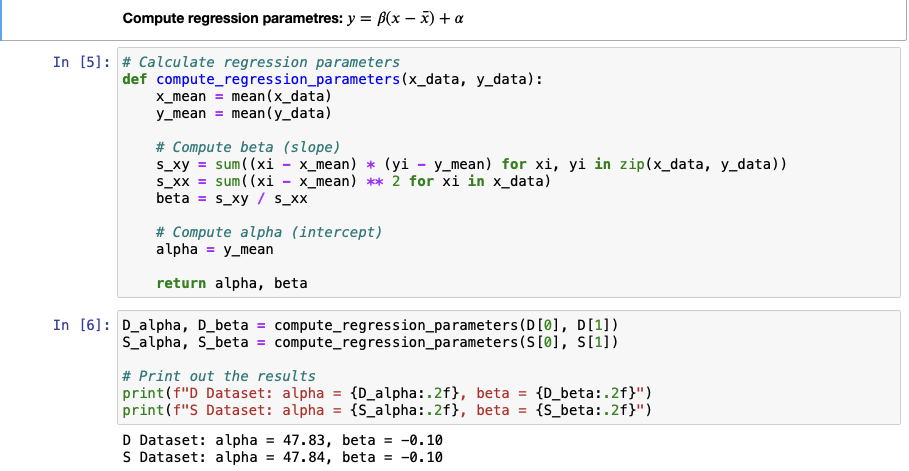
\includegraphics[width=0.8\textwidth]{regre.png}
    \end{figure} 
    \noindent \textbf{As a result,} we have regression parametres $\alpha$ = 47.83, $\beta$ = $-0.10$; $a$ = 47.84, $b$ =$-0.10$
    \\
    (c) Further we compute the confidence interval,
    \begin{figure}[H]
        \centering
        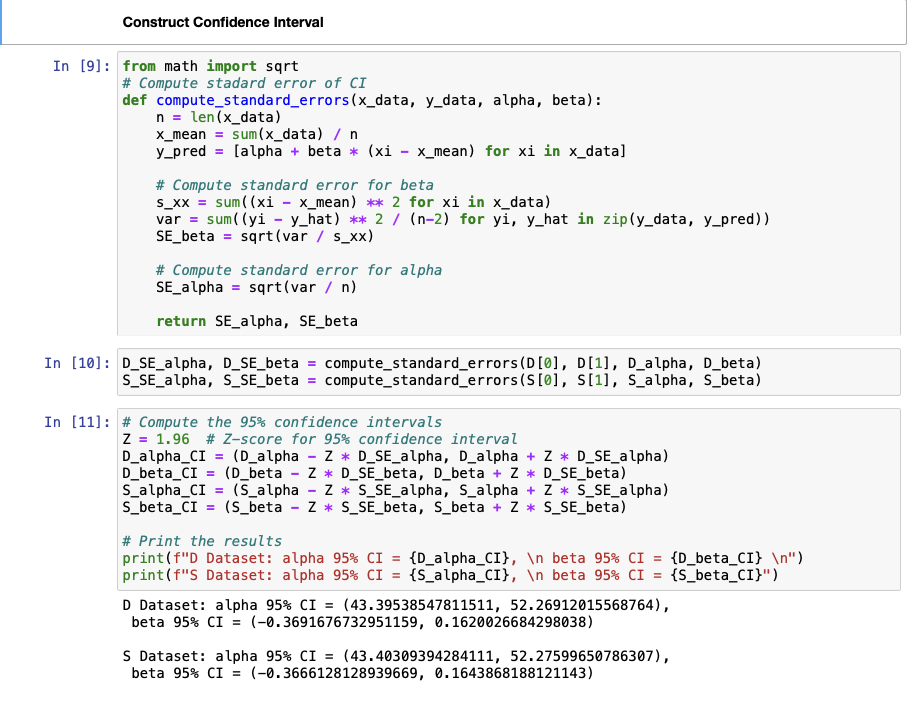
\includegraphics[width=0.8\textwidth]{ci_code.png}
    \end{figure} 
    \noindent \textbf{As a result, we have the confidence interval of each parametre as:} 
    \begin{table}[H]
        \centering
        \begin{tabular}{|l|c|c|c|c|}
        \hline
    Parametres  & $\alpha$          & $\beta$           & $a$              & $b$              \\ \hline
    CI          & (43.40, 52.27)    & ($-0.37$, 0.16)   & (43.40, 52.28)   & ($-0.37$, 0.16)    \\ \hline
    \end{tabular}
    \end{table}
    \noindent (d) Based on parametres of stastistics above, these two datasets are really similar.\\
    (e) To construct scatterplots for the datasets,
    \begin{figure}[H]
        \centering
        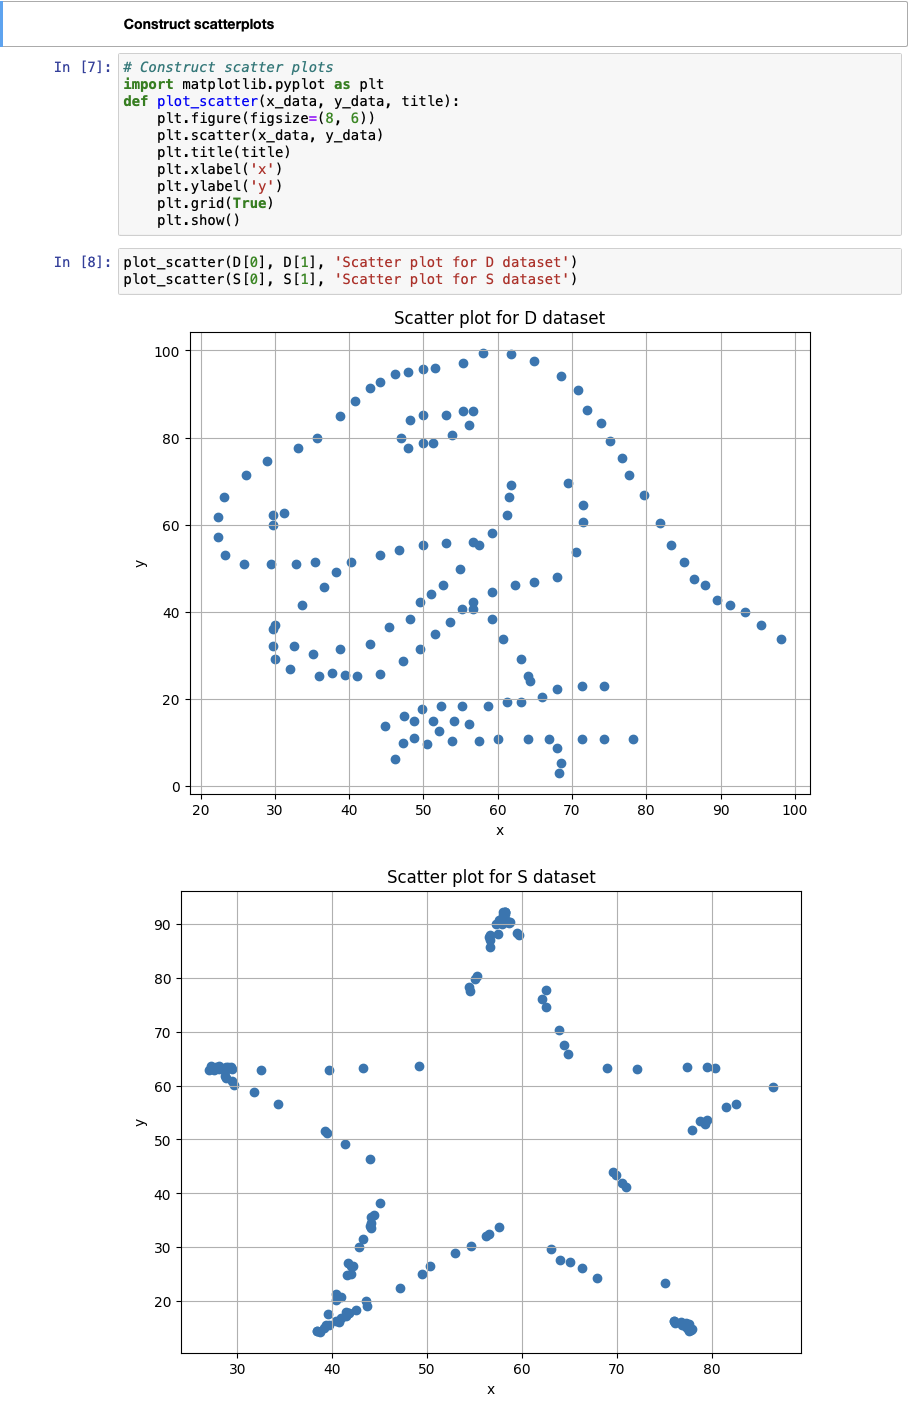
\includegraphics[width=0.8\textwidth]{scatter.png}
    \end{figure} 
    \noindent \textbf{Haha, it is really amazing $:\;)$ }\\
    (f) The two datasets are so alike in given parametres but quite different in scatter plots.
    That is, though specific parametres could reflect some characteristics of the given stastistic, it is still part of it instead of the whole. \\
\end{problem} 

% Problem 4
\begin{problem}
    \\
    By executing \textbf{r} codes as follows:
    \begin{figure}[H]
        \centering
        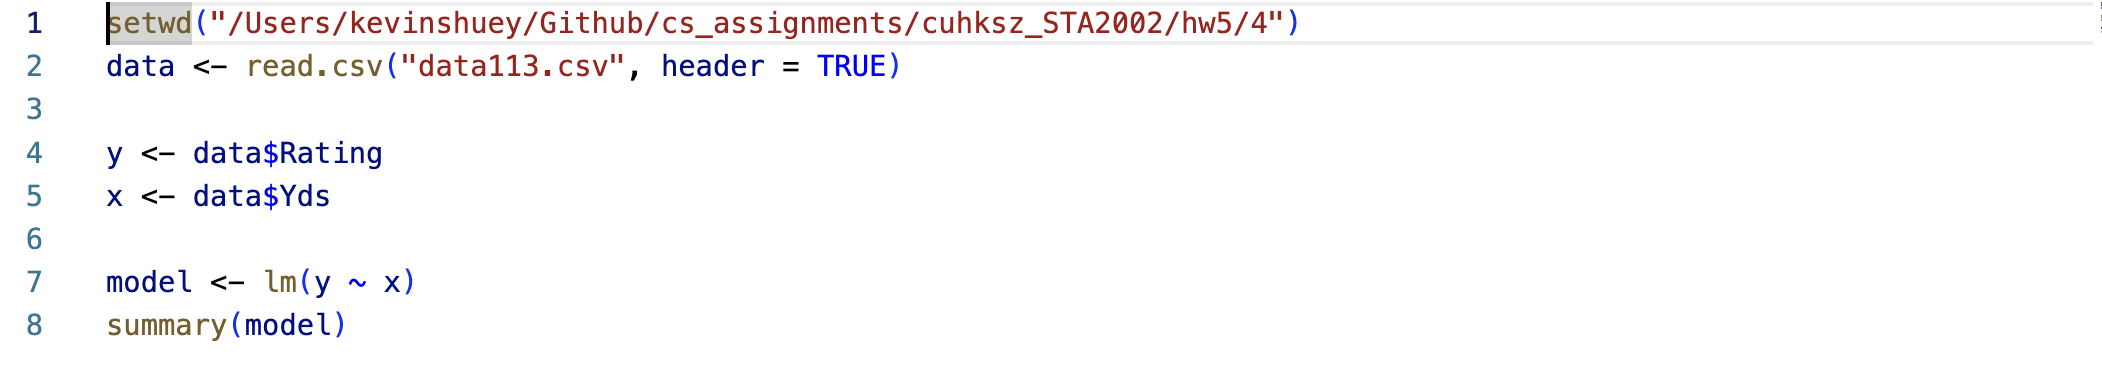
\includegraphics[width=0.8\textwidth]{lm_code.png}
    \end{figure} 
    We get comprehensive information like:
    \begin{figure}[H]
        \centering
        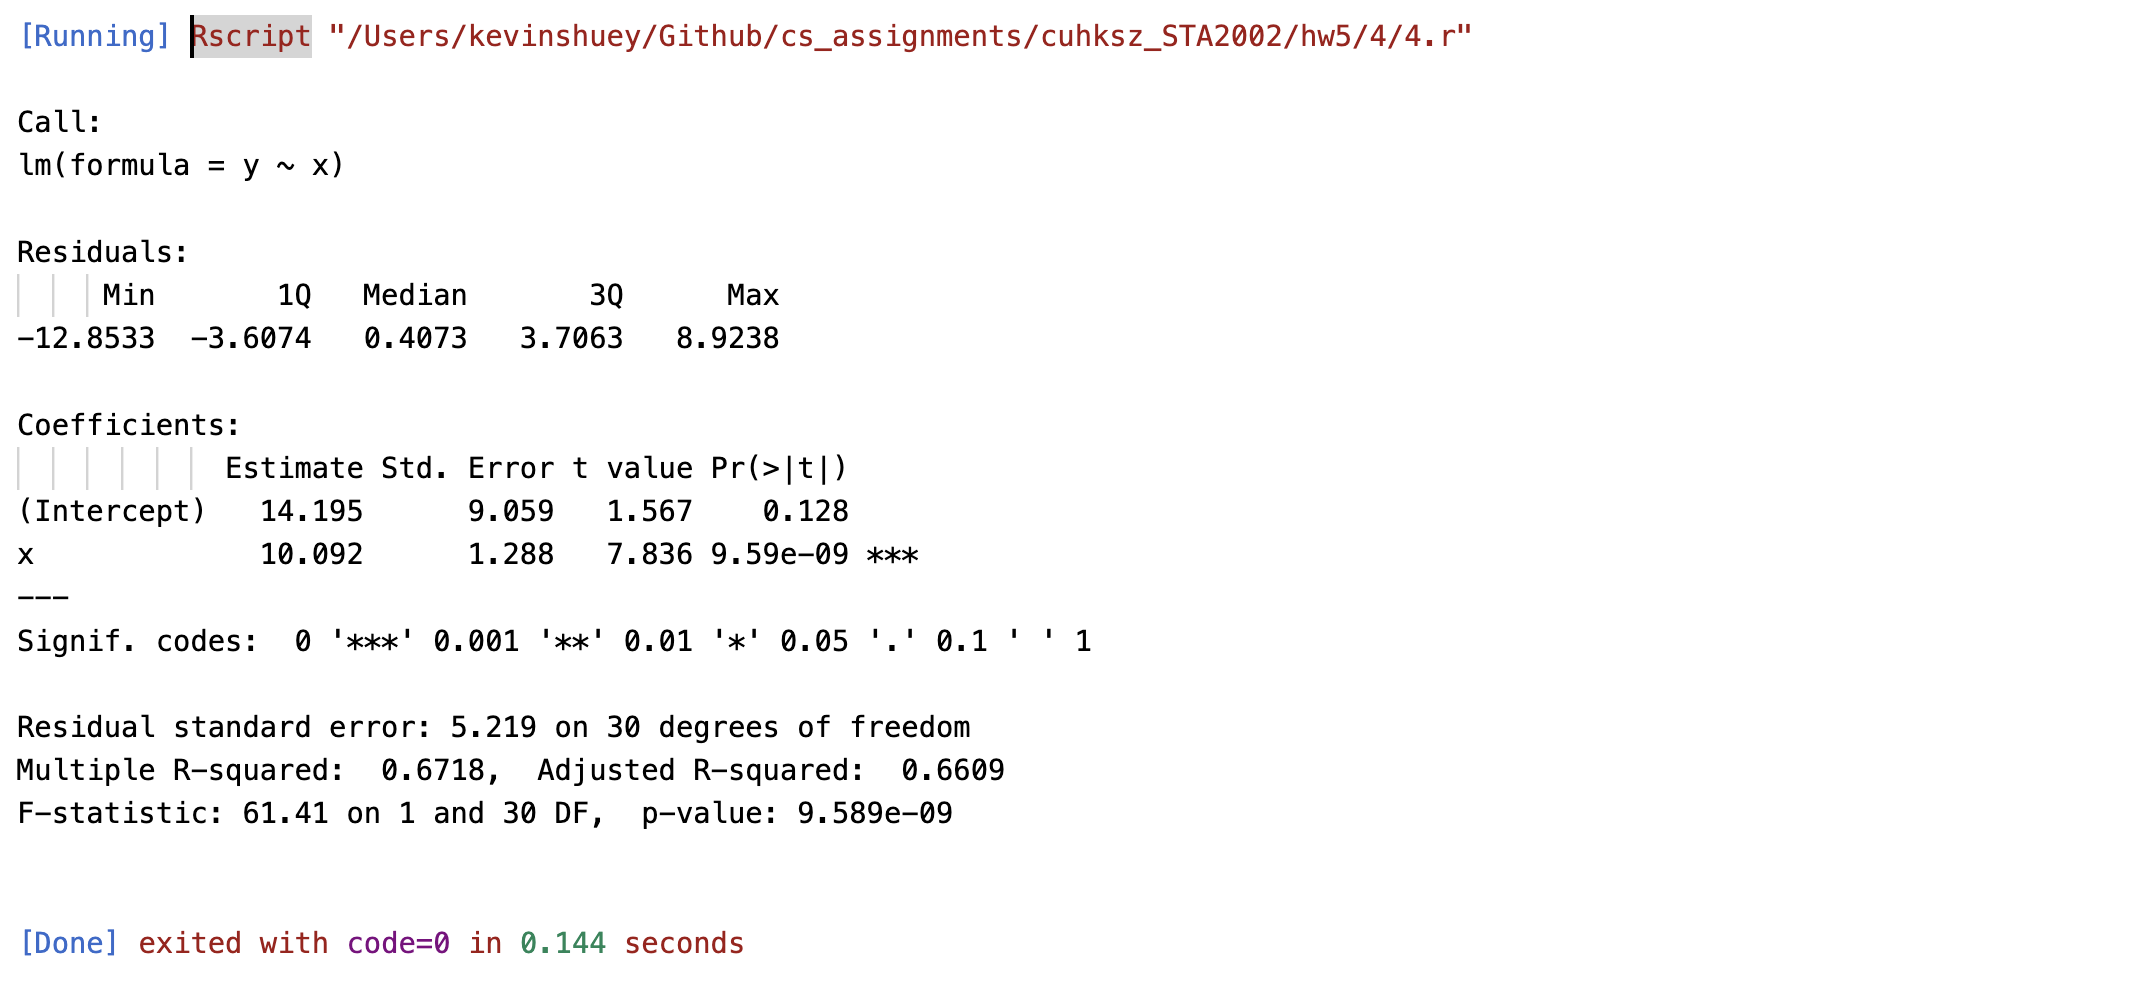
\includegraphics[width=0.8\textwidth]{lm_result.png}
    \end{figure} 
    \noindent Then we answer following questions:\\
    (\textbf{I} - a) According to the summary above, the \textbf{slope} $i.e.$ the coefficient of $x$, is 10.092; the \textbf{intercept} is 14.195; 
        the \textbf{estimate of} $\mathbf{\sigma^2}$ is $5.219^2 = 27.238$ . Here is the plot of $ \mathbf{y = 10.092 x + 14.195}$:
        \begin{figure}[H]
            \centering
            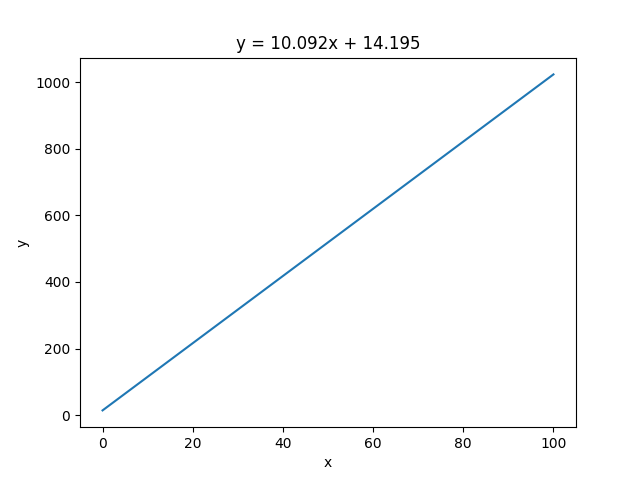
\includegraphics[width=0.5\textwidth]{fig_2.png}
        \end{figure} 
    \noindent (\textbf{I} - b) For a quarterback averages 7.5 yards per attempt $i.e.$ $x = 7.5$, 
    $$\mu_y = 10.092 \times 7.5 + 14.195 = 89.885$$
    \textbf{As a result, the estimate of mean rating is 89.885.} 
    \\
    (\textbf{I} - c) With a decrease of 1 yard per attempt, it will result in \textbf{a decrease of 10.092 yards}.
    \\
    (\textbf{I} - d) To reach an increase in mean rating by 10 points, it should \textbf{generate an increase in the average yards per attempt of 
    \;$\frac{10}{10.092} = 0.9909$} .
    \\ \\
    (\textbf{II} - a) The \textbf{r} results above has stated:
    $$ t_0 = \frac{\hat{\beta_1} - \beta_{1,0}}{\sqrt{\hat{\sigma}^2 / S_{xx}}} 
           = \frac{10.092 - 0}{\sqrt{27.238 / 16.4220}}= 7.836 > t_{0.01/2, \; 32-2} = 2.750,$$
    with p-value $$ \mathbf{p} = 9.59 \times 10^{-9} << 0.01$$
    Thus we reject the hypothesis. Meanwhile, the p-value is so small that there must be significant influence of $x$ to $y$ in slope.
    \\
    (\textbf{II} - b) As shown above by \textbf{r} results, the \textbf{standard error} for the slope is 1.288, and the one for the intercept is 9.059 .
    \\
    (\textbf{II} - c) Suppose we test $H_0: \beta_1 = 10$ versus $H_1: \beta_1 \neq 10$, \\
    First we calculate $$ S_{xx} = \sum_{i=1}^{n} (x_i-\bar{x})^2 = 16.4220$$
    Then we have t-value $$ t_0 = \frac{\hat{\beta_1} - \beta_{1,0}}{\sqrt{\hat{\sigma}^2 / S_{xx}}} 
                                = \frac{10.092 - 10}{\sqrt{27.238 / 16.4220}} = 0.0714 < t_{0.01/2, \; 32-2} = 2.750,$$
    thus we fail to reject the hypothesis.\\
    \textbf{As a result, it is reasonable to believe $\beta_1 = 10$ .}
    \\ \\
    (\textbf{III} - a) We still have $n = 32$ and  $\alpha =0.05$. \\
    For the slope $\beta_1$, we have
    $$ \hat{\beta_1} - t_{\alpha/2}(n-2)\sqrt{\frac{\hat{\sigma}^2}{S_{xx}}} \leq \beta_1 
            \leq \hat{\beta_1} + t_{\alpha/2}(n-2)\sqrt{\frac{\hat{\sigma}^2}{S_{xx}}}$$
    Specifically,
    $$ 10.092 - 2.042\sqrt{\frac{27.238}{16.4220}} \leq \beta_1 \leq 10.092 + 2.042\sqrt{\frac{27.238}{16.4220}}$$
    \textbf{As a result, we have a confident interval for $\beta_1$ of $\mathbf{(7.462, 12.722)}$.}
    \\
    (\textbf{III} - b) For the intercept $\beta_0$, we have
    $$ \hat{\beta_0} - t_{\alpha/2}(n-2)\sqrt{\hat{\sigma}^2 (\frac{1}{n}+\frac{\bar{x}^2}{S_{xx}})} \leq \beta_0
            \leq \hat{\beta_0} + t_{\alpha/2}(n-2)\sqrt{\hat{\sigma}^2 (\frac{1}{n}+\frac{\bar{x}^2}{S_{xx}})}$$
    Specifically,
    $$ 10.092 - 2.042\sqrt{27.238 \times (\frac{1}{32} + \frac{6.9978^2}{16.4220})} \leq \beta_0 
            \leq 10.092 + 2.042\sqrt{27.238 \times (\frac{1}{32} + \frac{6.9978^2}{16.4220})}$$
    \textbf{As a result, we have a confident interval for $\beta_0$ of $\mathbf{(-8.407, 28.591)}$.}
    \\
    (\textbf{III} - c) The mean rating at 8.0 is
    $$ \mu_{Y|x_0=8.0} = 10.092 \times 8.0 +14.195 = 94.931$$
    \textbf{As a result, the specific mean rating is 94.931 .}
    \\
    (\textbf{III} - d) For the rating, we have
    $$\hat{\mu}_{Y|x_0 = 8.0}-t_{\alpha/2}(n-2)\sqrt{\hat{\sigma}^2 (\frac{1}{n}+\frac{(x_0-\bar{x})^2}{S_{xx}})} \leq \mu_{Y|x_0 = 8.0} 
            \leq \hat{\mu}_{Y|x_0 = 8.0}+t_{\alpha/2}(n-2)\sqrt{\hat{\sigma}^2 (\frac{1}{n}+\frac{(x_0-\bar{x})^2}{S_{xx}})}$$
    Specifically,
    $$94.931 - 2.042\sqrt{27.238 \times (\frac{1}{32} + \frac{1.00438^2}{16.4220})} \leq \mu_{Y|x_0 = 8.0}  
    \leq 94.931 + 2.042\sqrt{27.238 \times (\frac{1}{32} + \frac{1.00438^2}{16.4220})}$$
    \textbf{As a result, we have a confident interval for $\mu_{Y|x_0 = 8.0} $ of $\mathbf{(91.687, 98.175)}$.}
\end{problem} 

% Problem 5
\begin{problem}
    \\
    \\
    By executing \textbf{r} codes as follows:
    \begin{figure}[H]
        \centering
        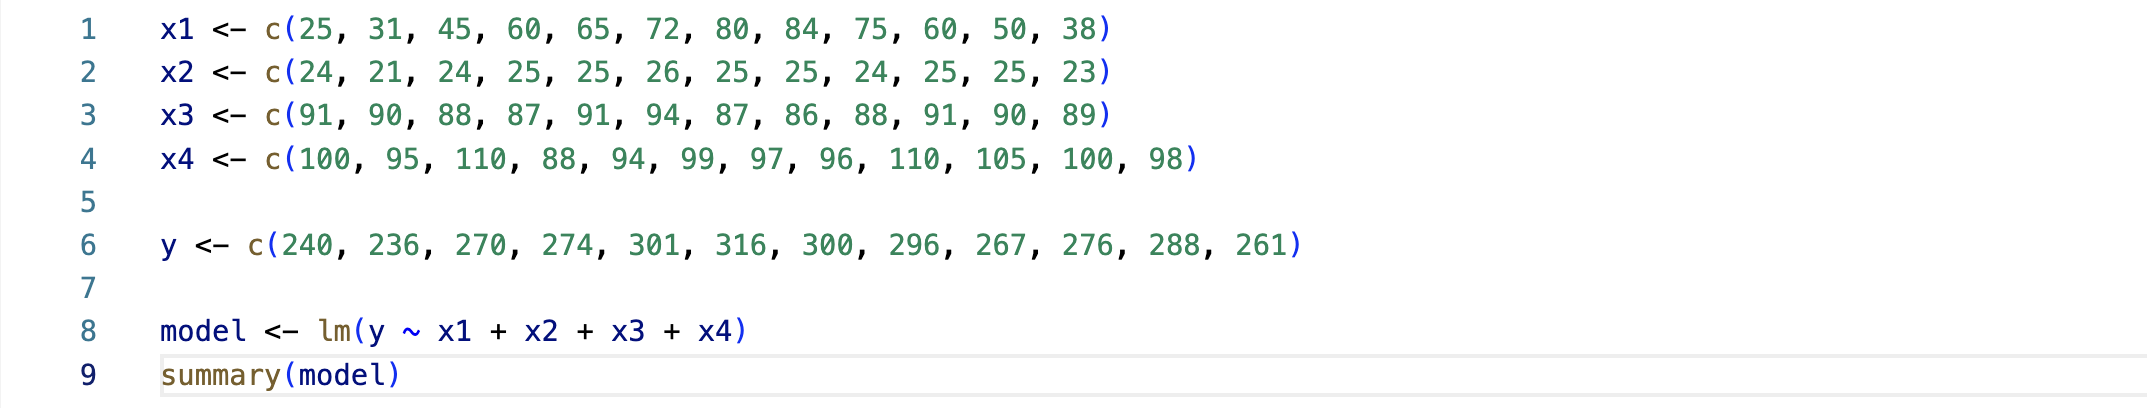
\includegraphics[width=0.8\textwidth]{lm_code2.png}
    \end{figure} 
    \noindent We get comprehensive information like:
    \begin{figure}[H]
        \centering
        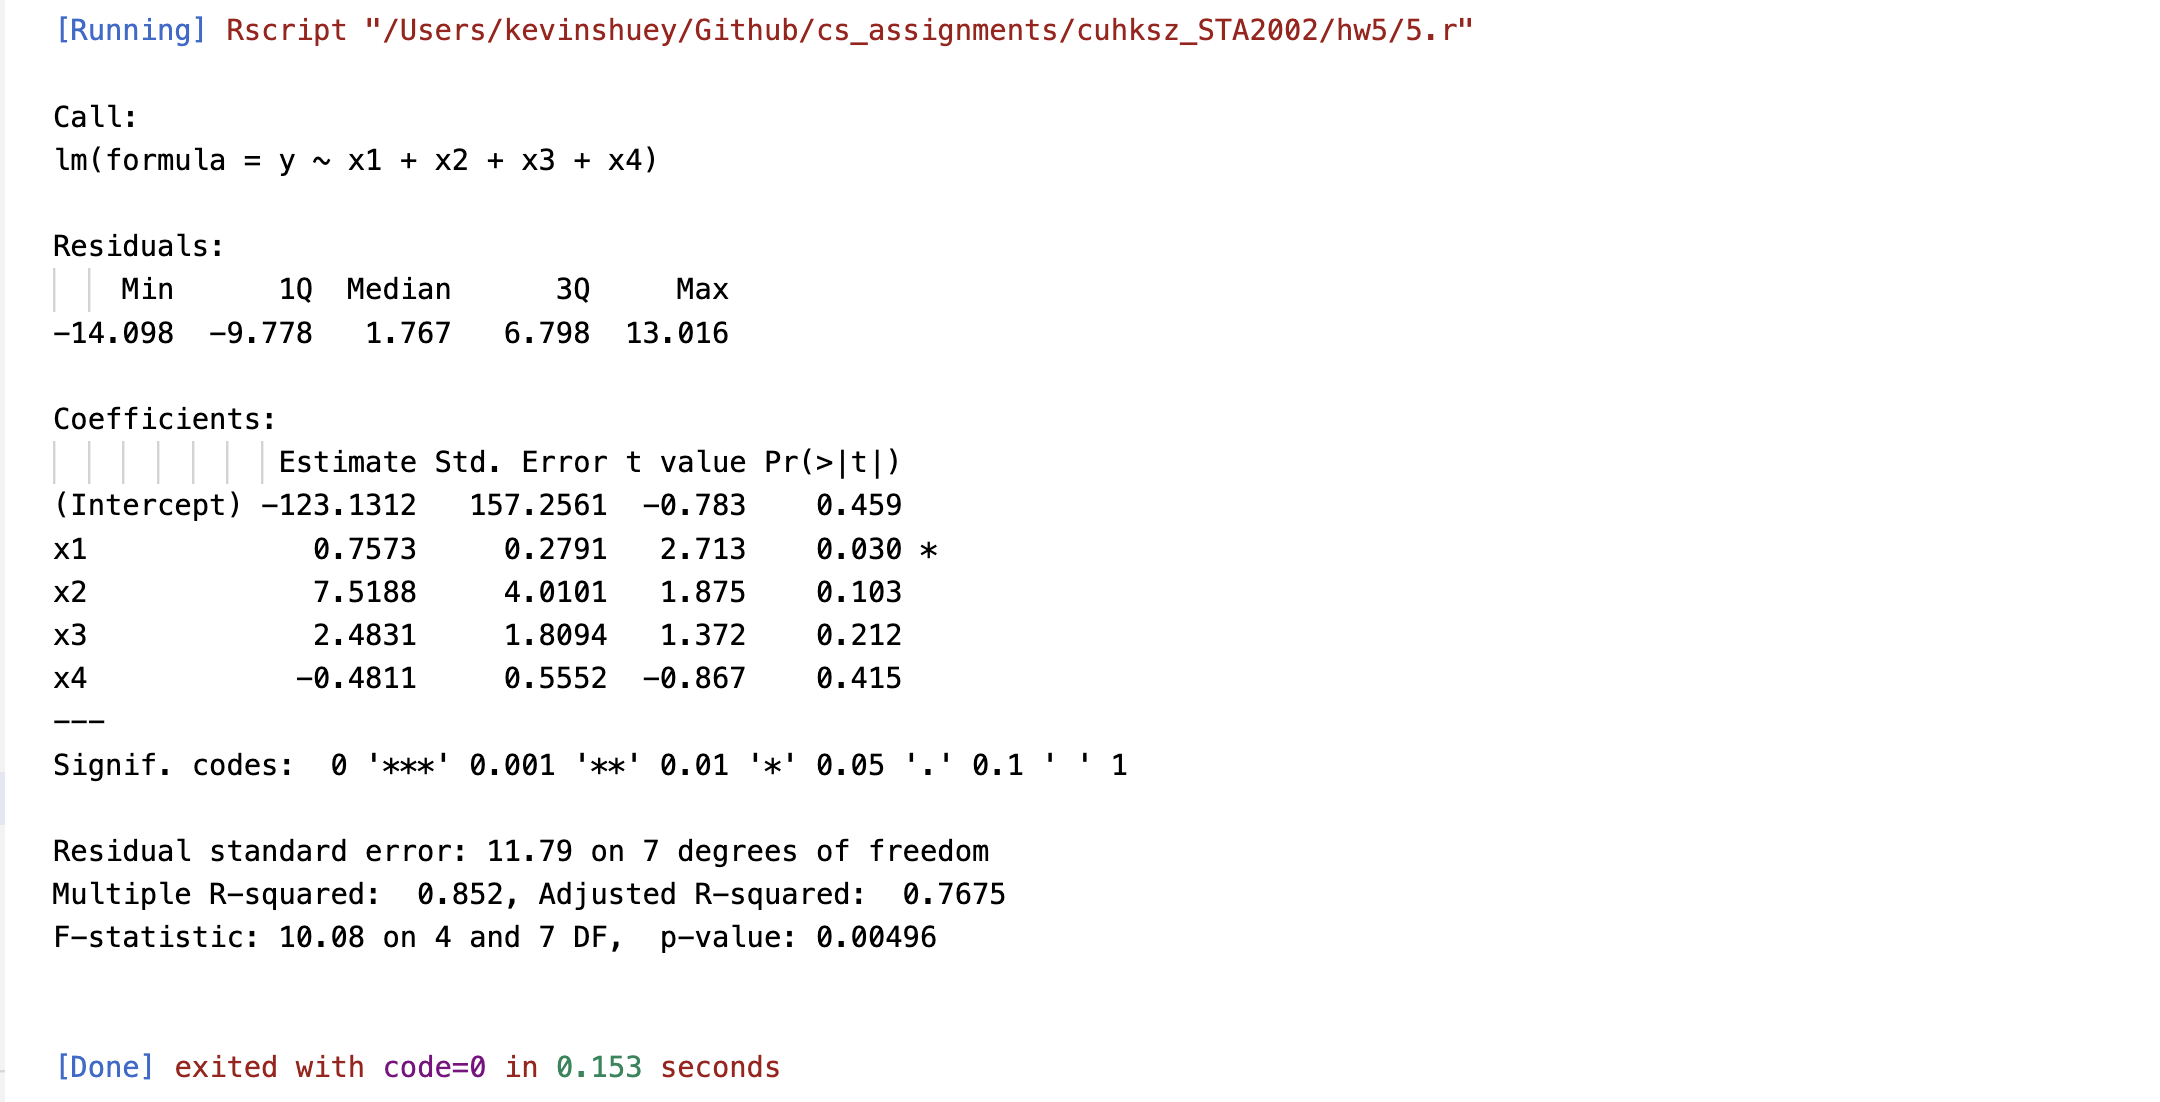
\includegraphics[width=0.8\textwidth]{lm_result2.png}
    \end{figure} 
    \noindent Then we answer following questions:\\
    (a) We construct a model like:
    $$ y = 0.7573 \cdot x_1 + 7.5188 \cdot x_2 + 2.4831 \cdot x_3 - 0.4811 \cdot x_4 - 123.1312 $$
    (b) Based on \textbf{r} results,
    $$ \hat{\sigma^2} = 11.79^2 = 139.0041$$
    (c) The \textbf{standard errors} for the coefficient of $x_1, x_2, x_3, x_4$ and the intercept are 0.2791, 4.0101, 1.8094, 0.5552 and 157.2561 respectively.
    They are NOT estimated with the same precision, as \textbf{they have different standard errors}. \\
    (d) For the given value,
    $$ y = 0.7573 \times 75 + 7.5188 \times 24 + 2.4831 \times 0.9 - 0.4811 \times 98 - 123.1312 = 69.2045$$
    \textbf{As a result, we predict the power consumption to be 69.2045.}
    \\ 
\end{problem} 
--------------------------------------------------\textbf{End of Homework 5} ------------------------------------------------
\end{document} 

